\documentclass[10pt,conference,compsocconf]{IEEEtran}
%\documentclass[journal]{IEEEtran}
\usepackage{amsmath, amsthm, amsfonts, amssymb}
\usepackage{graphicx}
\usepackage{multirow}
\usepackage{enumerate}
\usepackage[table,xcdraw]{xcolor}
\usepackage{amsmath}
\usepackage{diagbox}
\usepackage{bm}
\usepackage{algorithmic,algorithm}
\usepackage{etoolbox}
\usepackage{color,xcolor}
\usepackage{booktabs}
%\usepackage{caption}
\usepackage{subcaption}
\usepackage{hyperref}
%\usepackage{gensymb}

\usepackage{array}
\usepackage{makecell}

\renewcommand\theadalign{bc}
\renewcommand\theadfont{\bfseries}
\renewcommand\theadgape{\Gape[1.5pt]}
\renewcommand\cellgape{\Gape[1pt]}
\newcommand{\wz}{{\color{white}0}}

\renewcommand{\arraystretch}{1.25}


\begin{document}
\title{CIVIL-459 Deep Learning for Autonomous Vehicles -- Project Report}

\author{
  Tanguy Lewko, Chengkun Li, Yifeng Chen, Aoyu Gong\\
  \textit{\'Ecole Polytechnique F\'ed\'erale de Lausanne, Switzerland}
}

\maketitle

\section{Introduction} \label{sec:Introduction}
In this project, we developed a detector and a tracker that were later used to implement a person-following algorithm on a Loomo robot. The algorithm was further tested during the Tandem race. The main challenge is that our algorithm should be effective even in hard conditions, for instance, when the target object is not in the frame or obstructed by other objects. This project is divided into three milestones: detection, tracking, and implementation on the robot.


\section{Milestone 1 - Detection}
The goal of the first milestone is to detect, in real-time, a specific person, by using our own approach. We chose to detect a particular clothe: one group member's hat.

\subsection{The YOLOv5 Model}
Aiming to detect the hat, we chose YOLOv5 as the object detection algorithm due to its speed and accuracy \cite{YOLOv5doc}.
As shown in Figure \ref{fig:YOLOv5}, the architecture of YOLOv5 consists of three main parts: backbone, neck, and head.
The backbone is mainly based on \emph{Cross Stage Partial Network} (CSPNet) and \emph{Spatial Pyramid Pooling} (SPP) which extracts feature maps of different sizes by multiple convolutional and pooling layers.
The neck includes two parts: \emph{Feature Pyramid Network} (FPN) and \emph{Pixel Aggregation Network} (PAN).
The FPN conveys semantic features from higher feature maps to lower feature maps.
The PAN conveys localization features from lower feature maps to higher feature maps.
The head is used to predict targets of different sizes on feature maps.
The model consists of four architectures: YOLOv5s, YOLOv5m, YOLOv5l, and YOLOv5x.
In this milestone, YOLOv5s was trained and tested due to its smallest and fastest model.

\begin{figure}[!ht]
	\centering
	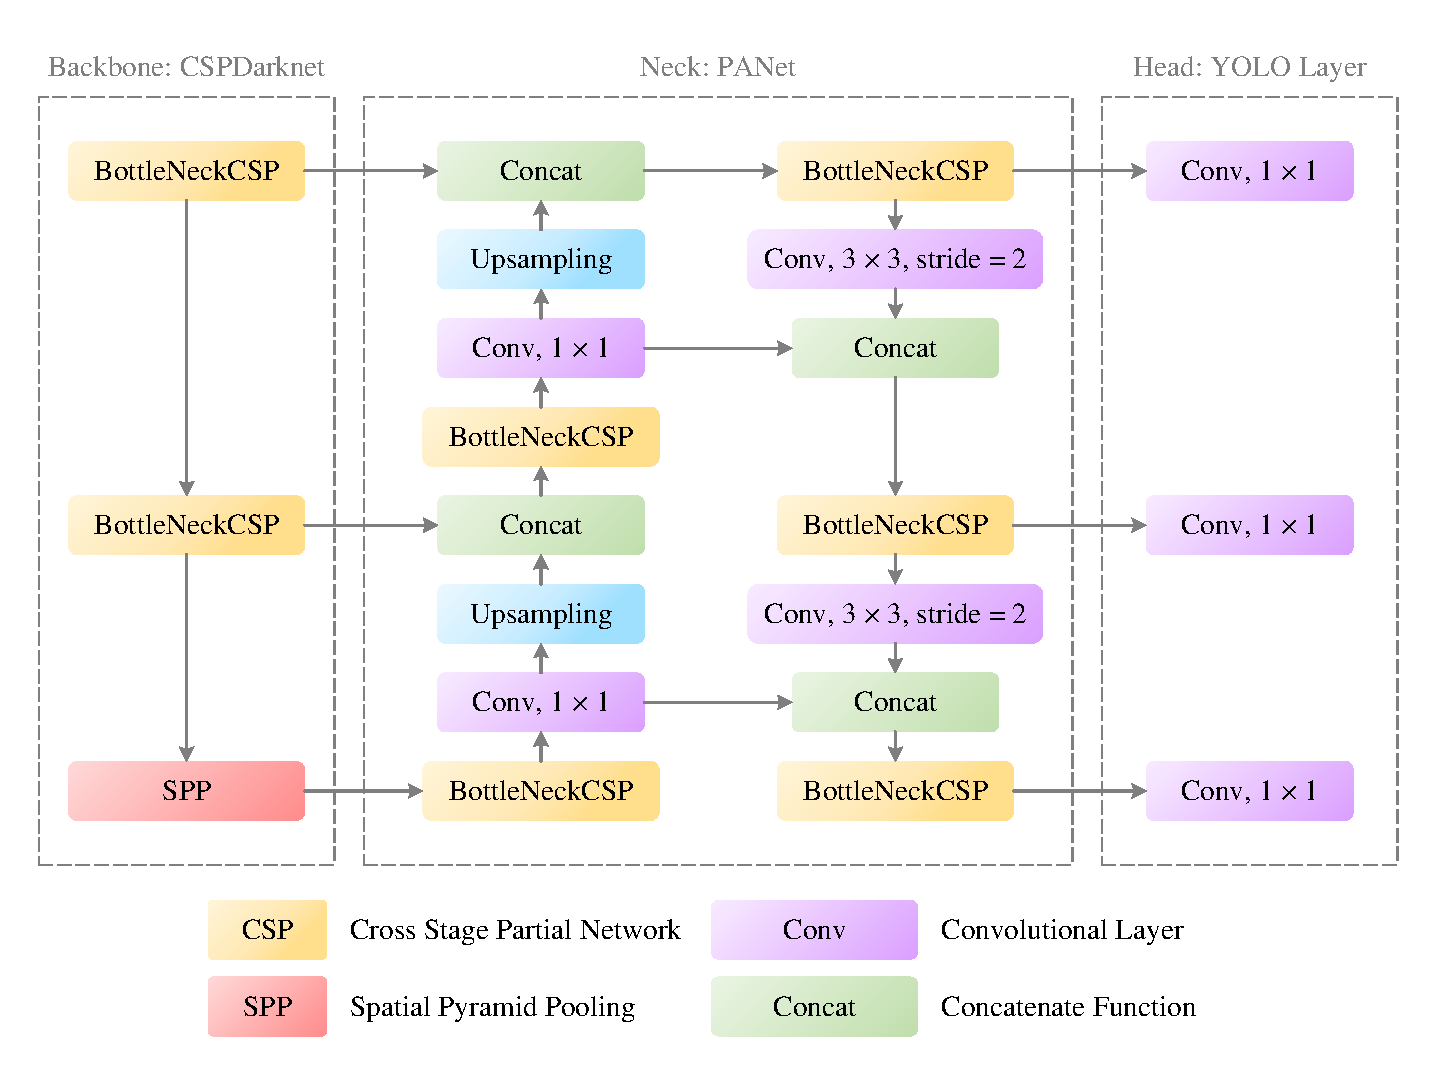
\includegraphics[width=0.9\linewidth]{./Image/YOLOv5.pdf}
	\caption{The architecture of YOLOv5.}
    \label{fig:YOLOv5}
\end{figure}

\subsection{Dataset}
The dataset for the object detection contains 1166 images of one group member wearing the hat in multiple different places, such as campus, parks, museums, subways, streets, shops, etc.
When taking these images, we changed the distance, light, directions, and obstructions as much as possible.
We also took into account different angles and focal lengths of the camera.
Then, we labeled the hat on all these images by using \href{https://roboflow.com/}{Roboflow}.
To adapt to the architecture of YOLOv5, we resized all images to the size of $640 \times 640$ pixels.
They were further divided randomly into the training, validation, and testing dataset, consisting of $816$, $225$, and $125$ images respectively.
After that, we implemented the following steps to generate three new images from every training image, including randomly cropping, rotating it between $-15^{\circ}$ and $+15^{\circ}$, changing its saturation and brightness between $-25\%$ and $+25\%$, and applying mosaic.
The augmented training dataset consisted of $2448$ images.

\subsection{Result Analysis}
Then, we trained YOLOv5s on our dataset. The training results are provided in Appendix \ref{sec:TrainingResults}. We chose this architecture because its inference speed is really fast and its results are ideal. The training part was really easy to do, so what we have learned in this milestone is how to create a good dataset, and train it with already existing algorithms. Our results using this algorithm are robust. We often have high confidence when detecting: greater than 0.9, and extremely few false detections with a confidence threshold of 0.5 (in the final race we set it to 0.6). Since we know there will be only one person of interest wearing the hat on a frame, we also decided to only keep the bounding box with the highest confidence. Images with no hat labeled were added to avoid false positives when detecting. Figure \ref{det} presents the results on some of our images from the testing dataset. We observe that even in Figure \ref{fig:Hard}, where the hat is far away, obstructed behind an object, and under bad light conditions, the hat is still detected with high confidence.

\begin{figure*}%[!ht]
  \centering
  \begin{subfigure}{0.23\textwidth}
    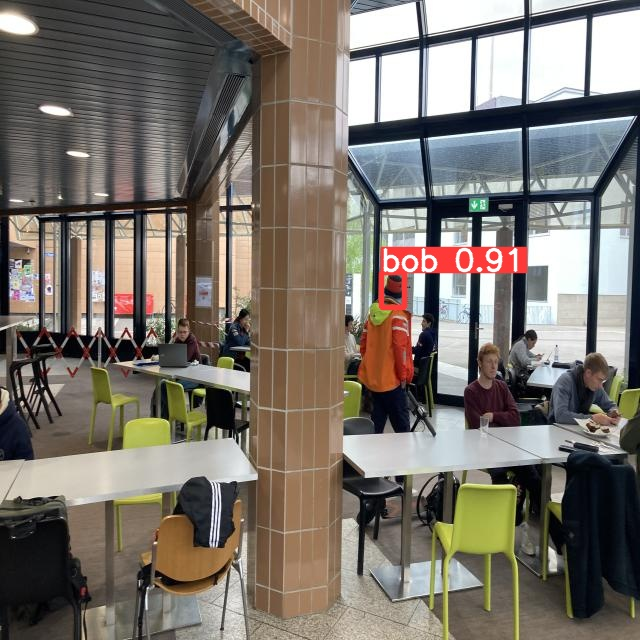
\includegraphics[width=\linewidth]{Image/bob8.jpg}
    \caption{On campus (CO).}
  \end{subfigure}
  \hfil
  \begin{subfigure}{0.23\textwidth}
    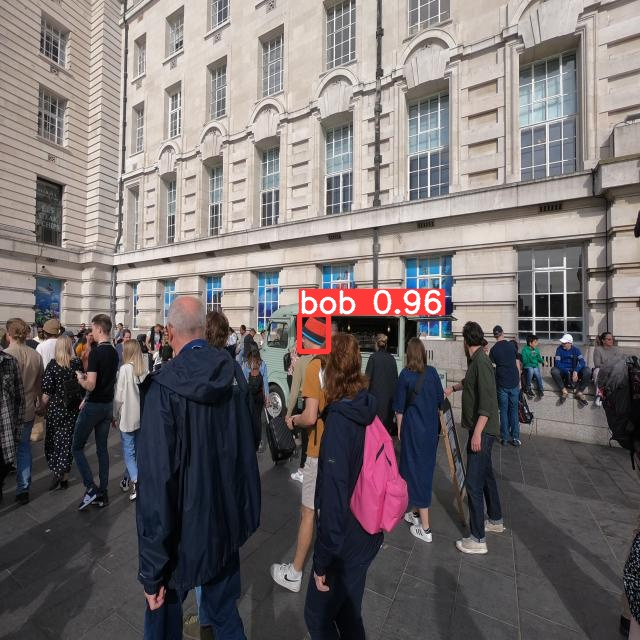
\includegraphics[width=\linewidth]{Image/bob4.jpg}
    \caption{In a street.}
  \end{subfigure}
  \hfil
  \begin{subfigure}{0.23\textwidth}
    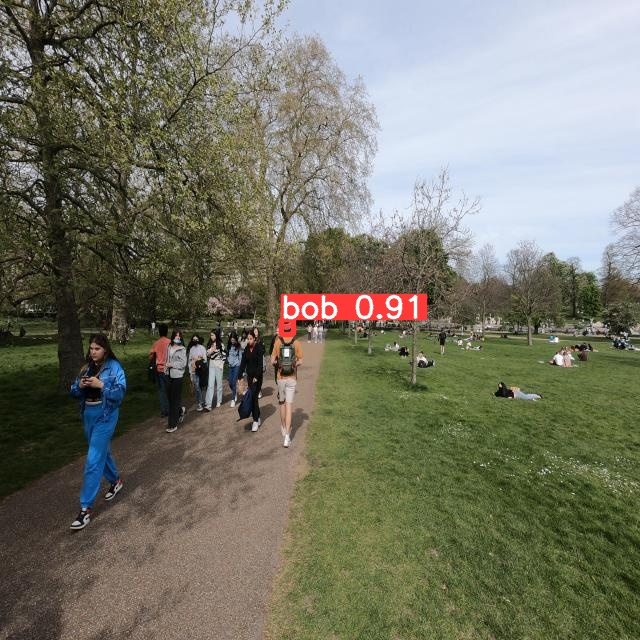
\includegraphics[width=\linewidth]{Image/bob10.jpg}
    \caption{In a park.}
  \end{subfigure}
  \hfil
  \begin{subfigure}{0.23\textwidth}
    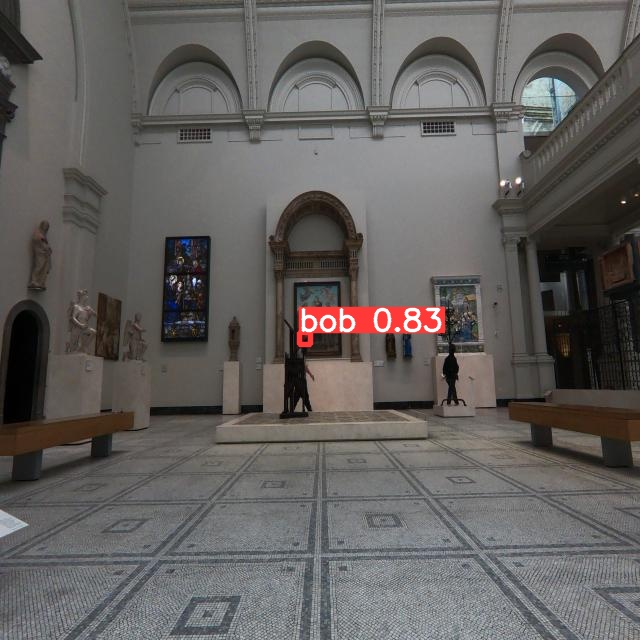
\includegraphics[width=\linewidth]{Image/bob7.jpg}
    \caption{In a museum.}
    \label{fig:Hard}
  \end{subfigure}
  \caption{Detection with testing images taken in different places.}
  \label{det}
\end{figure*}


\section{Milestone 2 - Detection + tracking}
The second milestone was about developing a tracker to track the person of interest. In order to do so, we used the Deep SORT algorithm combined with YOLOv5s.

\subsection{The Deep SORT Algorithm}
To track the person of interest, we chose the Deep SORT algorithm due to its robustness for real-time tracking \cite{wojke2017simple}.
It takes advantage of YOLOv5 in accurately detecting objects with two classic methods: the Kalman filter and Hungarian algorithm.
Moreover, it integrates a deep association metric derived from a convolutional neural network, which results in high robustness from occlusion, change in viewpoint, etc.

\begin{figure}[!ht]
	\centering
	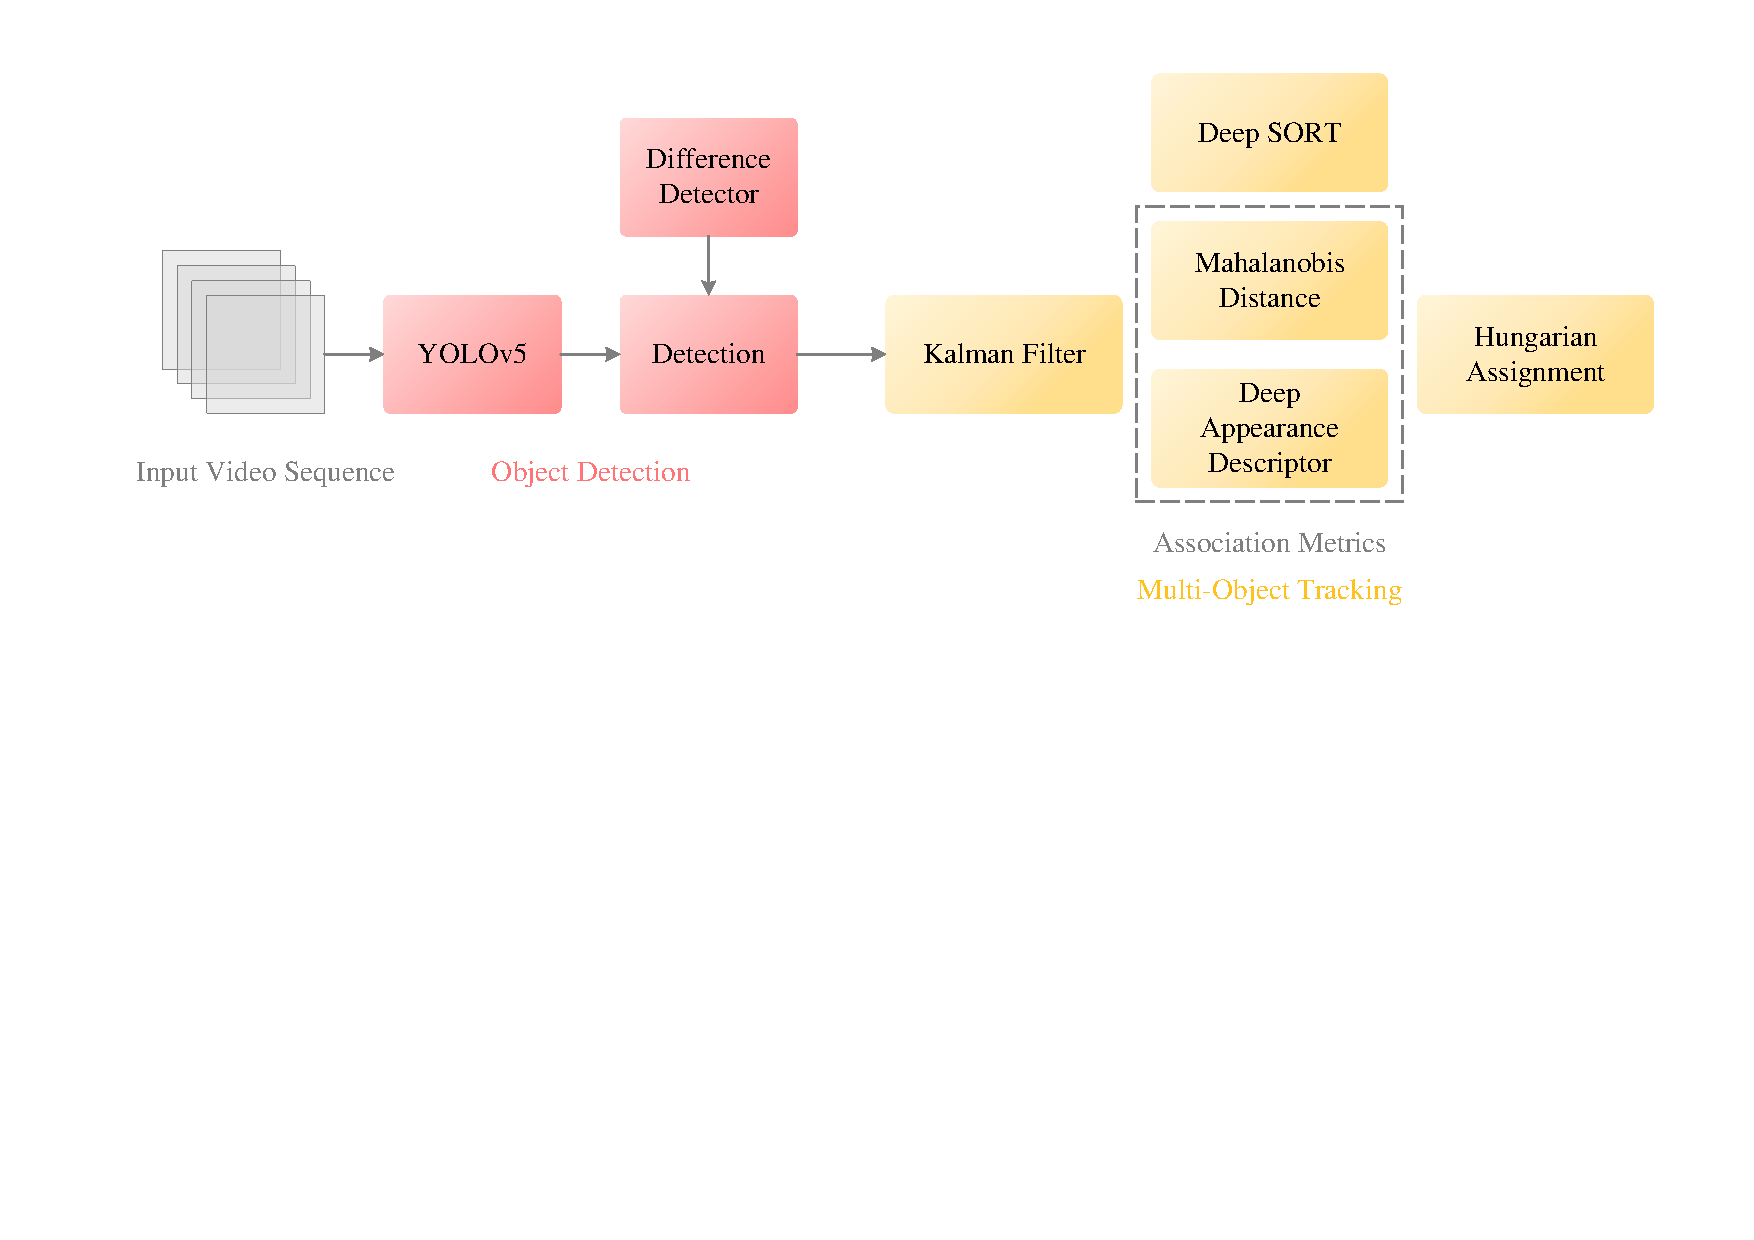
\includegraphics[width=0.9\linewidth]{Image/DeepSort.pdf}
	\caption{The architecture of deep SORT.}
    \label{fig:deepSORT}
\end{figure}

\subsection{Initialization and Tracking}
 The tracker is initialized when the hat is detected. Then, YOLOv5 is used to detect the bounding box of the person which has the biggest intersection area with the bounding box of the hat. The bounding box of this person is then fed to the tracker, and the person of interest can remove the hat and be tracked.

\subsection{Result Analysis}
Our tracker handles well with scenarios where the person of interest leaves the frame, and when that person comes back the tracker could immediately rediscover and track the location of the person. The main weak point of our tracker is that if a person is partially obstructed, by another object for a long time, the tracker might identify another person as the person of interest (this happened a few times during tests with many people in front of the camera). To solve that, we thought about using the first bounding box to track instead of the last one. It solves the problem but we ended up with less good performance in general when the person is moving fast. So, we decided to stick to the first method. Maybe using a combination of the first and the last bounding boxes could give us better results but we did not do it before the milestone 2 deadline.

\section{Milestone 3 - Tandem race}
\subsection{The Choice of the Algorithm}
The final milestone is to implement our algorithm on the Loomo robot.
Given that our detection algorithm works perfectly well and was robust owing to the good dataset we spent much time creating, we decided to only use detection but not tracking. Indeed, even if the tracker is working well, we still have to take the risk that it might change the person of interest in some rare cases, which we hope to avoid for the race. 
Not only that, it saves the time for re-initialization of the tracking algorithm if the tracker loses the target.

\subsection{The Novelty of the Algorithm}
To add smoothness to our person-following algorithm, we decided that if the person of interest was not detected for an intermediate frame (usually happens when the light condition changes drastically), keep the last bounding box for five frames before making the robot stop. This allows us to simulate a zero linear constant Kalman filter for a short time in case there is nothing detected. It worked pretty well in practice given the fact that the manipulator of the robot rarely gets out of the camera's field of view.

\subsection{The Result of the Tandem Race}
Since we created the good dataset, chose the appropriate algorithm, and guided the robot well during the race, we achieved a great result in the race. For the race against the clock, we took \textbf{49.58 seconds} to finish it, ranking second among all teams. For the final competition, we achieved the \textbf{first prize}!




\section*{Acknowledgements}
The authors thank Prof. Alexandre Alahi, Parth Kothari, George Adaimi, Mohammadhossein Bahari, Saeed Saadatnejad, and other TAs for providing the robot, computing resources, and careful guidance, as well as for the well-organized race.

\newpage
\onecolumn

\bibliographystyle{IEEEtran}
\bibliography{literature}

\begin{appendices}
\section{Training Results} \label{sec:TrainingResults}
%The training results are provided as follows.
\begin{figure*}[!ht]
  \centering
  \begin{subfigure}{0.24\textwidth}
    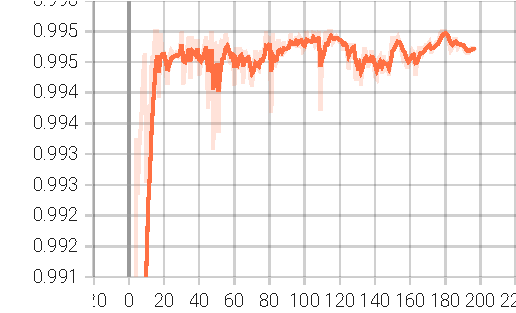
\includegraphics[width=\linewidth]{Image/metrics_mAP_0.5.pdf}
    \caption{mAP@.5}
  \end{subfigure}
  \hfil
  \begin{subfigure}{0.24\textwidth}
    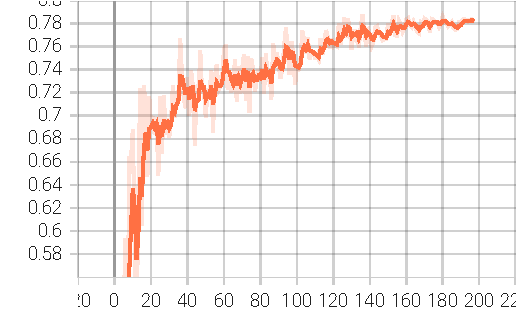
\includegraphics[width=\linewidth]{Image/metrics_mAP_0.5_0.95.pdf}
    \caption{mAP@[.5:.95]}
  \end{subfigure}
  \hfil
  \begin{subfigure}{0.24\textwidth}
    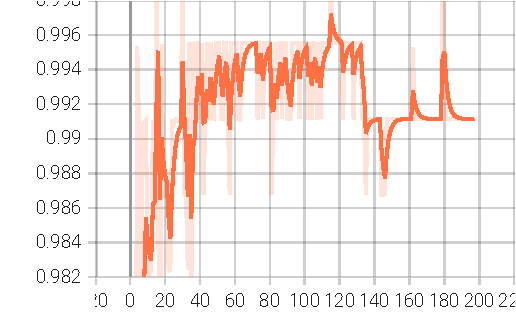
\includegraphics[width=\linewidth]{Image/metrics_precision.pdf}
    \caption{Precision}
  \end{subfigure}
  \hfil
  \begin{subfigure}{0.24\textwidth}
    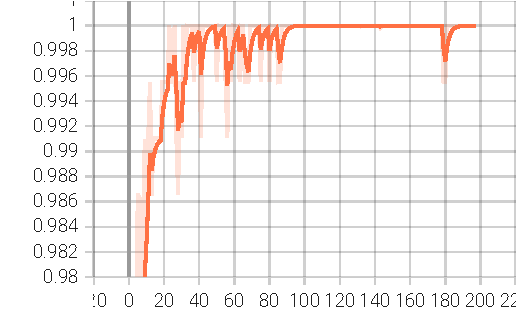
\includegraphics[width=\linewidth]{Image/metrics_recall.pdf}
    \caption{Recall}
  \end{subfigure}
  \caption{The four metrics as a function of the number of epochs.}
\end{figure*}

\begin{figure*}[!ht]
  \centering
  \begin{subfigure}{0.27\textwidth}
    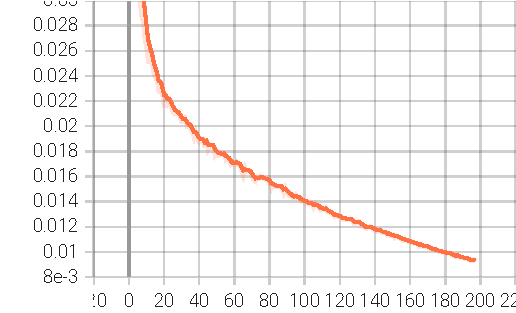
\includegraphics[width=\linewidth]{Image/train_box_loss.pdf}
    \caption{The bounding coordinates}
  \end{subfigure}
  \hfil
  \begin{subfigure}{0.27\textwidth}
    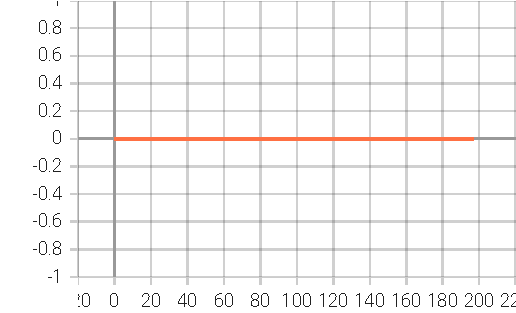
\includegraphics[width=\linewidth]{Image/train_cls_loss.pdf}
    \caption{The object confidence}
  \end{subfigure}
  \hfil
  \begin{subfigure}{0.27\textwidth}
    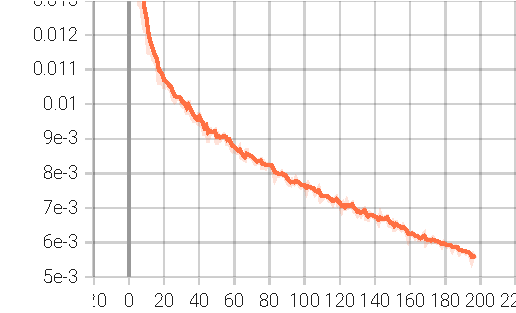
\includegraphics[width=\linewidth]{Image/train_obj_loss.pdf}
    \caption{The classification loss}
  \end{subfigure}
  \caption{The three losses as a function of the number of epochs.}
\end{figure*}

\section{Photos of the Tandem Race} \label{sec:TandemRace}
%The photos in Tandem Race are provided as follows.
\begin{figure*}[!ht]
  \centering
  \begin{subfigure}{0.4\textwidth}
    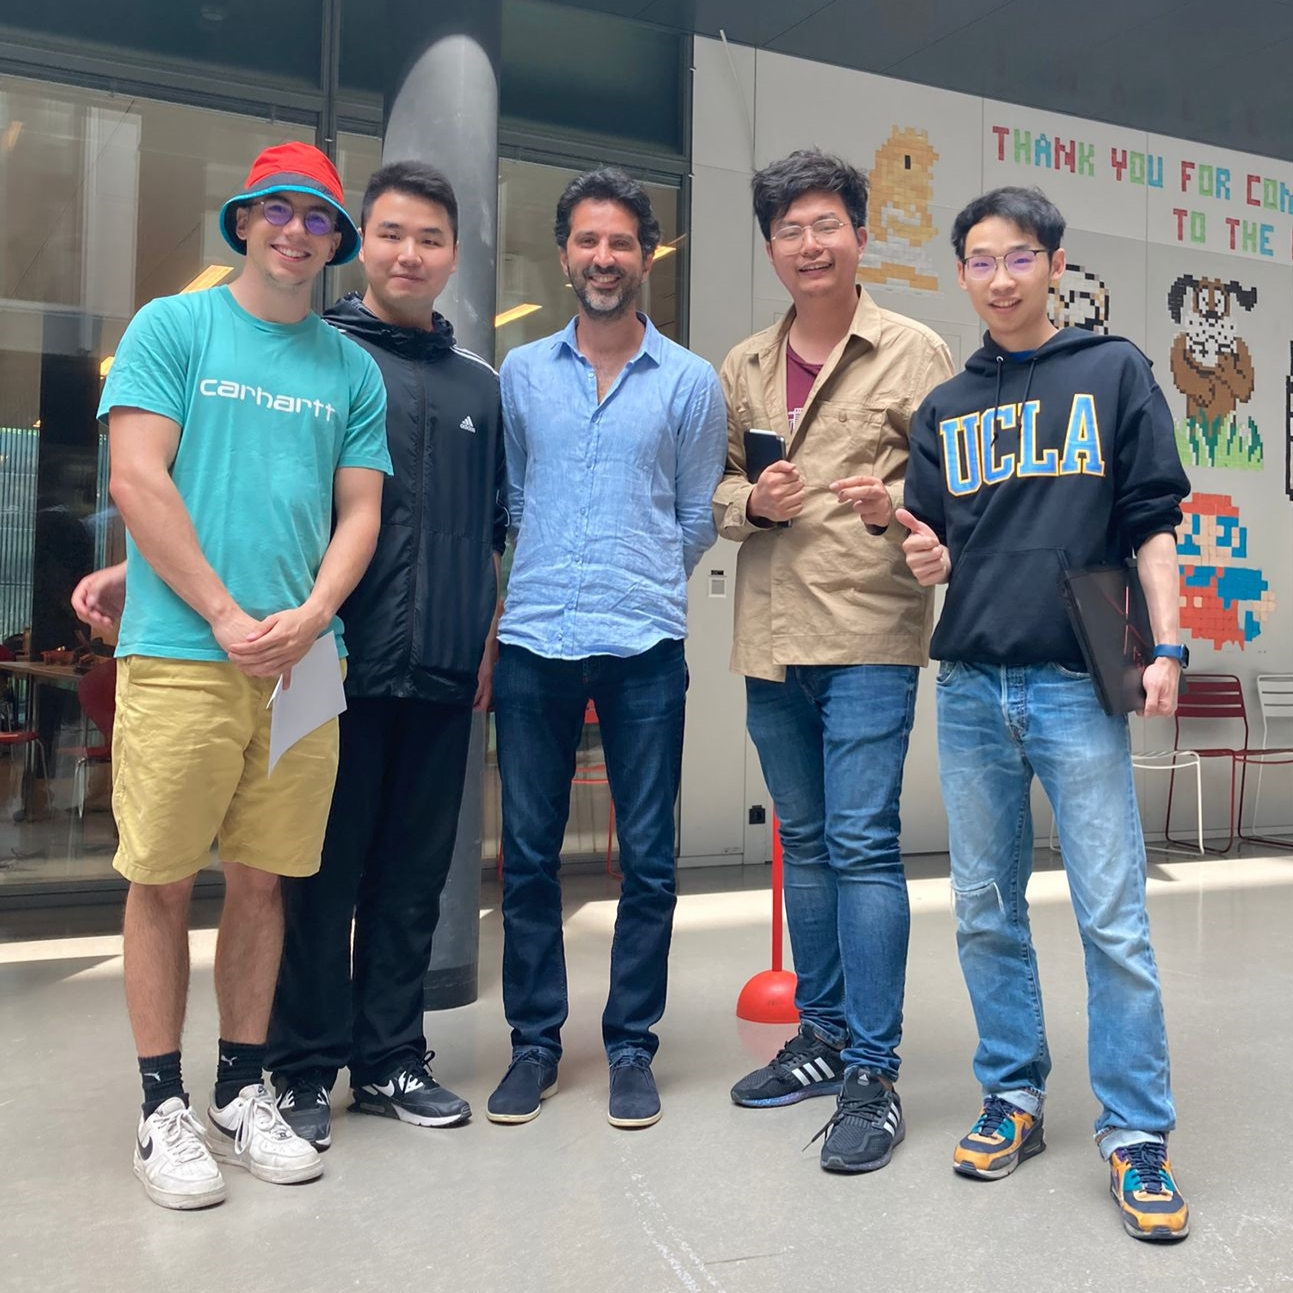
\includegraphics[width=\linewidth]{Image/Photo1.jpeg}
    \caption{Prof. Alexandre Alahi and group members.}
  \end{subfigure}
  \hfil
  \begin{subfigure}{0.4\textwidth}
    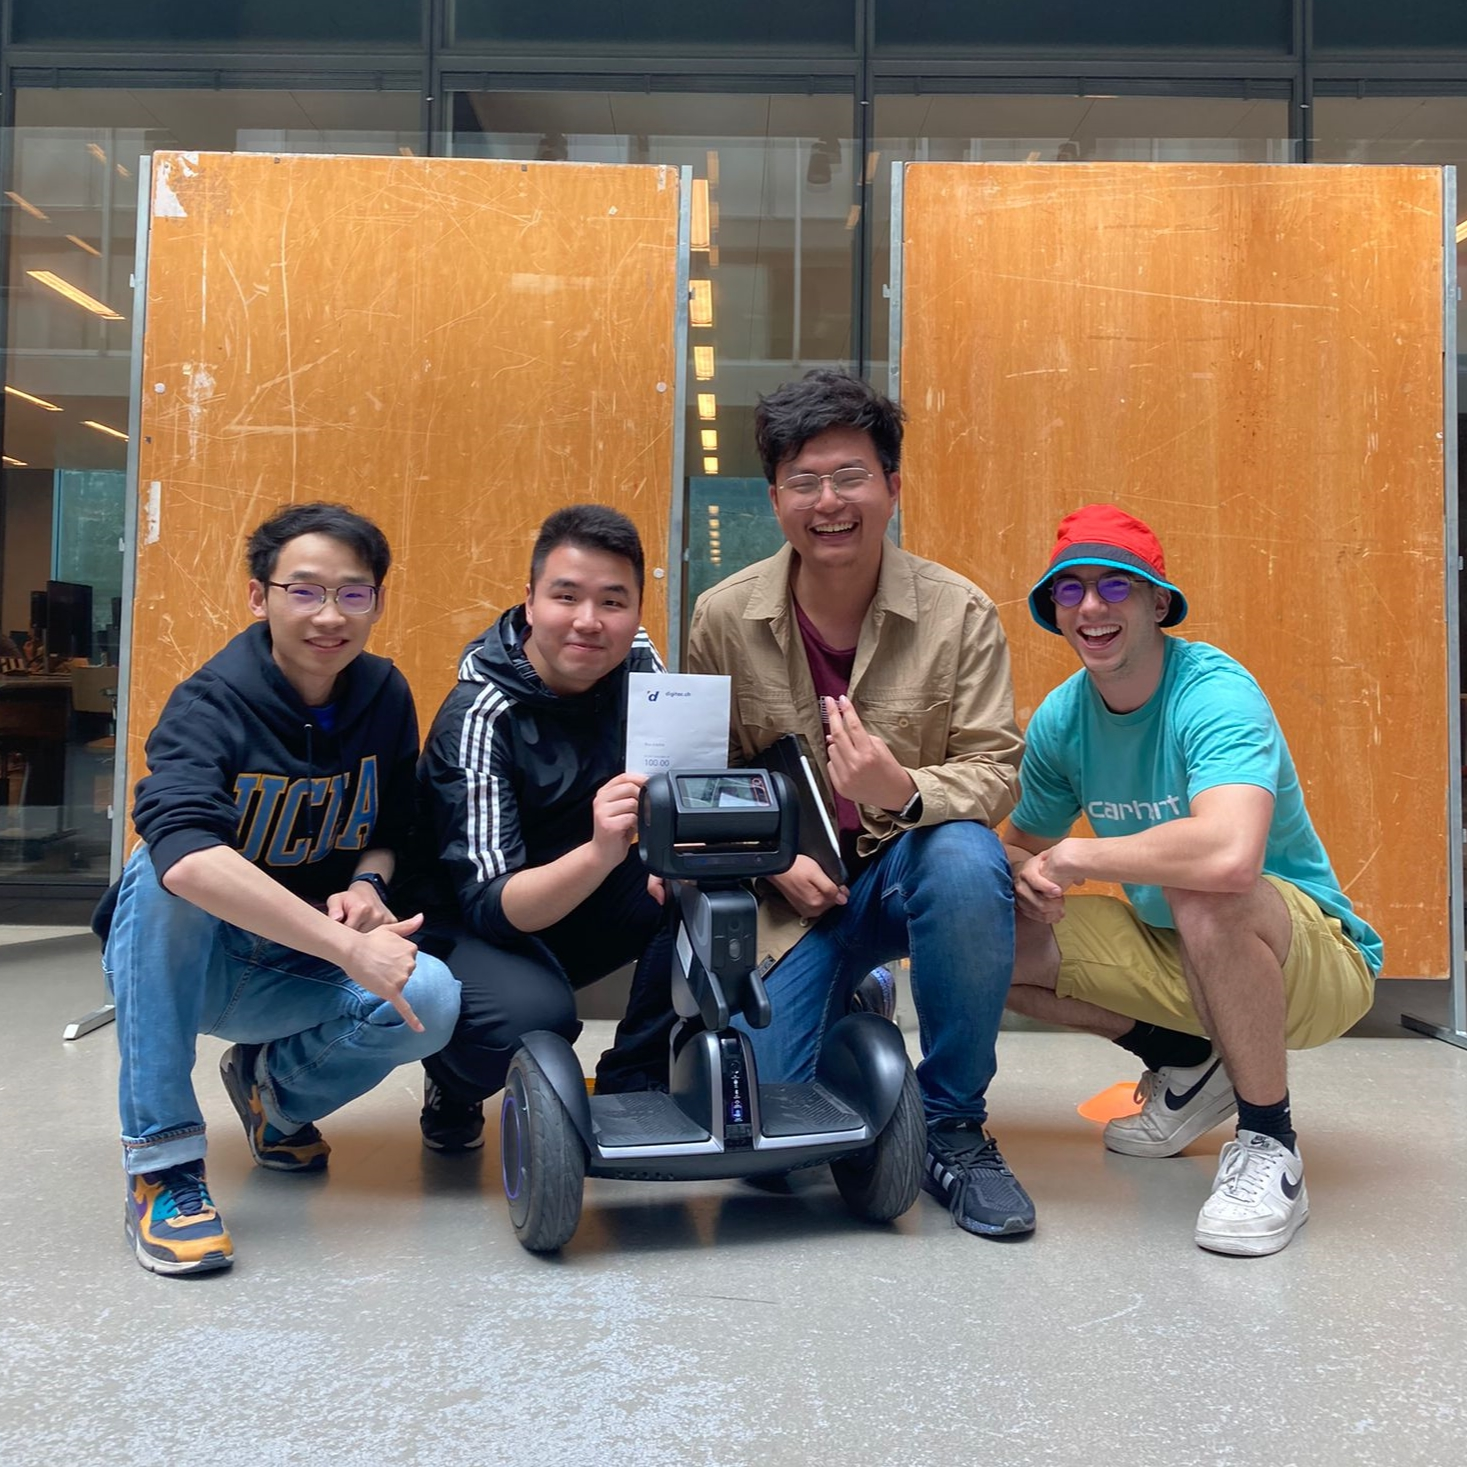
\includegraphics[width=\linewidth]{Image/Photo2.jpeg}
    \caption{Group members with the lucky robot.}
  \end{subfigure}
  \caption{The photos of the Tandem Race.}
\end{figure*}

\end{appendices}


\end{document}
